\documentclass[12pt]{article}
\usepackage{graphicx}
\usepackage[style=alphabetic, backend=biber]{biblatex}
\graphicspath{ {./images/} }

\addbibresource{figures.bib}

% Preamble
\setlength{\parindent}{0pt}

% Document Information
\title{Optimal Method of Ray Tracing Voxels with Hardware Acceleration in Real-Time}
\author{Srijan Dhungana}
\date{2024}

% Begin Document
\begin{document}

% Title Page
\maketitle
\clearpage

% Table of Contents
\tableofcontents
\clearpage

\section{Motivation}

My first introduction to ray tracing was when NVIDIA announced their RTX series GPUs in 2018.
The idea of simulating light rays in real-time was unreal to me and the results were stunning.
I wanted to make my own hardware ray tracer and so I was introduced to computer graphics.
I have always been fascinated by the aesthetics of voxels based games and I wanted to combine the two.
However, when researching, I found that there was not much information on the fastest method to ray trace a voxel scene with hardware acceleration.
This essay is an attempt to answer that question.

% Introduction
\section{Introduction}

\subsection{Ray Tracing}

Ray tracing is a method to calculate where a given ray (line), intersects
with the environment. This is useful to simulate light rays because of how light behaves. It is used in film
production, video games, optics, medical imaging, architectural visualization,
and many other fields. Physically light rays bounce in the environment, thus
ray tracing is used to calculate the position of intersection where a light ray
hits the environment. Then the programmer is free to repeat the process
and simulate the ray bouncing off into other directions. This process is a
highly parallelizable process, thus it is perfectly suited for GPUs which have
thousands of cores. However, due to how computationally expensive the
process is, it is not feasible to do in real-time without dedicated hardware
acceleration. Due to those limitations, it was only used in non-real-time
applications such as film production and pre-rendered graphics. Hardware
acceleration ray tracing was introduced in 2018 by Nvidia. Since then, ray
tracing has been possible in real-time and further supported by AMD and
Intel GPUs. This has allowed real-time applications to leverage ray-tracing

\subsection{Voxels}

Voxels are a way to represent 3D data. It is similar to pixels in 2D images,
but in 3D space. Essentially, voxels are cubes that are located in 3D space.
They are used in medical imaging, simulations, and video games; they have
similar applications to ray tracing. Voxels are convenient, because they rep-
resent volumetric data, which is difficult to represent with polygons. For
example, a physics simulation of a fluid would be difficult to represent with
polygons, but easy with voxels. Each voxel can store data such as color,
density, temperature, etc. at each point in 3D space. The resolution of the
simulation can also be adjusted easily just by changing the size of the voxels.

\subsection{Research Question}

The research question is: What is the difference in performance between
purely hardware based voxel ray tracing and a mixed software-hardware approach in rendering?

\section{Background Information}

\subsection{Mathematics of Ray Tracing}
\subsubsection{The Ray Equation}

A ray is defined by a point and a direction. The equation of a ray is given by:

\begin{equation}
    R(t) = \vec{o} + t\vec{d}
\end{equation}

where $\vec{o}$ is the origin of the ray, $\vec{d}$ is the direction of the ray, and $t$ is the distance from the origin.
The function $R(t)$ gives the position of the ray at distance $t$ from the origin.
With this equation, we can start to calculate the point of intersection along the ray with a surface.

\subsubsection{The Intersection Function}

Whenever a ray intersects with a surface, the point of intersection is given by the equation:

\begin{equation}
    R(t) = I(t)
\end{equation}

where $I(t)$ is the intersection function of the surface. To locate the point of intersection,
solving for $t$ is necessary by equating the ray equation with the intersection function. 
If there are negative solutions for $t$, then the ray intersects with the surface. However, 
if $t$ is negative, then the intersection is opposite the direction of the ray, which is not usually desired,
so negative solutions are ignored. The closest hit is desired, so the smallest positive $t$ is chosen.

The intersection test has to happen for every object in the scene to determine the closest intersection.
This is computationally expensive for large scenes, so acceleration structures (AS) are used to decrease the number of intersection tests significantly.
These structures are usually bounding volume hierarchies (BVH) that subdivide the scene into smaller parts until the smallest primitives are reached.

\begin{figure}[h]
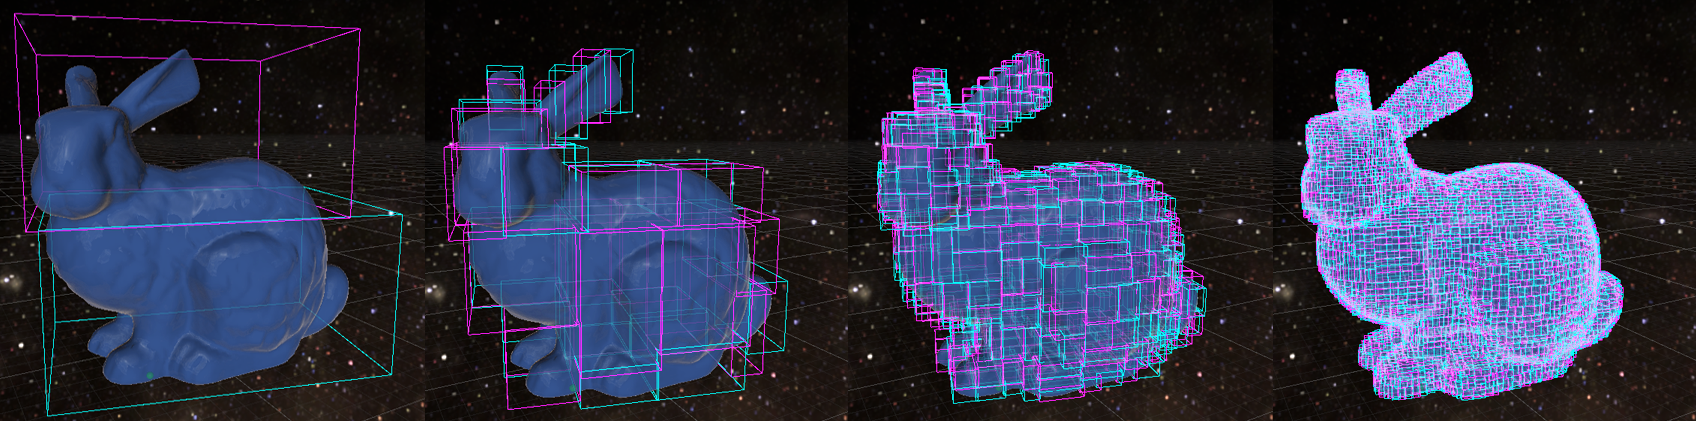
\includegraphics[scale=0.22]{BVH-Visualization}
\caption{Bounding Volume Hierarchy of a bunny form \parencite{Medium:BVH-Visualization}. The bunny is divided into smaller bounding volumes until the individual triangles are reached.}

\end{figure}

When a ray enters a bounding volume, the algorithm only has to test for intersections with the objects in that volume, which is much efficient.
The BVH is a non-trivial tree structure that is constructed every object in the scene and requires a lot of memory, because
it stores the volumes in addition to the objects.

\subsection{Ray Tracing Algorithm}

The ray tracing algorithm is a recursive algorithm that calculates the color of a pixel by tracing rays into the scene.
The scene has a virtual camera that acts like a real camera capturing photons but instead of capturing photons, it shoots rays
into the scene.
This is because a light source emits photons in unmeasurable quantities and it is impossible to simulate all of them and a typical scene has multiple light sources.
Additionally, not all photons reach the camera, so most of the computation is wasted.
When tracing from the camera, the algorithm can simulate the exact paths but it only simulates paths that reach the camera.

The algorithm is as follows for each pixel in the image:
\begin{enumerate}
    \item Calculate a ray direction for the pixel.
    \begin{itemize}
        \item This is dependent on the field of view, focal length, and many other factors such as a real lens.
    \end{itemize}
    \item Trace the ray into the scene and find the {\bf closest} intersection. If there is no intersection, then the ray hits the background.
          This could be the sky or a solid color that acts as ambient light.
    \item If the surface is emissive (light source), then the ray's color is a combination of the light source and the colors of the surfaces it hit along the way and the algorithm stops.
          If it is not emissive, then the ray absorbs some percentage of the surface's color and bounces in another
          direction and the algorithm repeats from step 2.
\end{enumerate}

This algorithm is repeated thousands of times for each pixel in the image and the result is a photorealistic image.
The reason it is repeated is that there can be thousands of paths that reach the camera bouncing from different combinations of surfaces.
Even then, the image is an approximation because the algorithm fails to simulate all the paths that reach the camera.

\subsection{GPU Architecture}

TODO: Explain how GPUs work and how they are used in ray tracing. Also some 3D vs 1D for SDFs maybe?

\section{Methods}
\subsection{Hardware Acceleration Structure Traversal}

To use an AS it needs to be constructed for the objects in the scene.
Unfortunately, acceleration structure generation is a black box in graphics APIs. 
The user supplies the object's primitives and the GPU driver constructs it.
These primitives are usually triangles or axis aligned bounding boxes (AABB).
AABBs are cuboids that are aligned in the x, y, and z axes.

Cubes can be represented as AABBs, so voxels can be represented as AABBs.
This is useful because the GPU can construct the AS without the user having to do it.
However, the AABBs are not inteded to use as voxels, instead they are a flexible way to enclose user defined objects.
For example, a smooth sphere would not be possible to represent using triangles, but there 
is an intersection function that would render a smoother sphere than triangles ever could.
AABBs are used to enclose the sphere and the GPU will notify the user for any potential hits with the sphere.
This can be done for anything as long as it's enclosed in an AABB.
Because of this, they are not optimized for the voxel use case, where there would be millions of
densely packed AABBs in a scene.

Additionally, the memory consumption is greater for AABBs than for voxels.
AABBs need 2, 3D vectors to represent the minimum and maximum points of the cuboid.


\subsection{Signed Distance Fields}
\subsection{Other Algorithms}

\section{Memory Consumption}

\section{Results}

\section{Conclusion}

\printbibliography

\end{document}